\pagestyle{fancy}
\headheight 20pt
\lhead{Ph.D. Thesis --- R. Woods}
\rhead{McMaster - Physics \& Astronomy}
\chead{}
\lfoot{}
\cfoot{\thepage}
\rfoot{}
\renewcommand{\headrulewidth}{0.1pt}
\renewcommand{\footrulewidth}{0.1pt}

\chapter{The Numerical Method}
\label{chap:method}
\thispagestyle{fancy}

The main goal of the algorithm presented in this chapter is to solve the radiative transfer equation. We prioritize the ability to deal with a large number of sources and computational speed over high accuracy, though we still insist equilibrium behavior be correct.

In order to accomplish this, we first start by dropping scattering to simplify the equations of RT. We also note that by summing radiation over all sources, we need not explicitly include emission in the equation. This means equation \ref{eq:combinedtransfer} simplifies down to equation \ref{eq:absorption}, which has the solution

\begin{equation}
\label{eq:absorptionsolution}
I_{\nu}(\mathbf{r}) = I_{\nu,0}e^{-\tau},
\end{equation}

where $I_{\nu,0}$ is the intensity from a particular source.

%In the absence of absorbing material, the problem of radiative transfer reduces down to that of gravity. As such, the tree-algorithm for calculating gravity can be used \citep{barnesHut86}.

In the absence of absorbing material, the optical depth is 0 and equation \ref{eq:absorptionsolution} implies that we need only sum over all sources. This problem is almost identical to gravity, and so we choose to use the same tree-based technique as gravity to solve it.

The tree-based gravity solver of \citet{barnesHut86} has become commonplace in astrophysical simulations \citep{wadsleyEt03}[cite codes that use it]. They scale well with the number of resolution elements ($N\log(N)$) and are easily tuned to the desired accuracy. It is also easily made parallel. For these reasons, we choose to implement a tree to perform radiative transfer.

Please note that following algorithm has been implemented in SPH. As such, we choose to refer to resolution elements as particles, as is common in SPH codes. However, the algorithm is not specific to SPH, and ``particle'' can be replaced with whatever represents the resolution element in another code.

%\begin{equation}
%\label{eq:gravitymoments}
%\Phi = \frac{G}{4\pi}\sum\limits_{n=0}^{\infty} \frac{1}{r^{(n+1)}}\int (r')^n P_n (\cos{\theta '}) \rho(\boldsymbol r') d\tau '
%\end{equation}

%\begin{equation}
%\label{eq:radiationmoments}
%F = \frac{L}{4 \pi r^2}
%\end{equation}

\section{Tree Data Structures}
\label{sec:treestruct}

In order to understand the radiative transfer algorithm that we are presenting, it is important to understand tree data structures.

In computer science, a tree is any data structure that stores data in a hierarchical way. Typically, the data is stored in a ``node'' or ``cell.'' Each node then has 1 or more ``child nodes'' that branch off from it, and each of those child nodes in turn has child nodes, and so on. In order to store simulation data in a tree, we simply need to partition the data in a hierarchical way. The easiest way to do this is to partition the simulation volume itself.

The entire simulation volume is stored in the ``root node'', or the top of the tree. We then partition the root node into a smaller unit. A common choice is an octree, which splits a cube into eight sub-cubes, or a binary tree, which splits a volume into two smaller volumes. In the former case, every node has eight children, while in the latter case, each node has two children. Note that all children with a common parent are referred to as siblings. While the algorithm we have developed is independent of tree-type, we will introduce it in the context of a binary tree, since this is what \textsc{Gasoline} uses.

Starting with the root node, the volume is split into two smaller volumes. In memory, particles are partitioned about the split value, which is an $\mathcal{O}(N)$ operation. The tree-build continues recursively, splitting each child node into smaller volumes. In a binary tree, it is common to choose your split value as either the midpoint of the longest axis in the volume, or the midpoint that gives an equal number of particles on either side. Both of these options are available to our RT algorithm. The splitting continues until a condition is met. Typically, this condition is that a volume contains less than a specified number of particles in it. A cell that meets this criteria will be at the bottom of the tree, and is called a ``leaf'' or ``bucket.''

During this process, a node can request average properties from the nodes beneath it, such as total luminosity, center of luminosity, and so on. Once the tree has been partitioned down to leaves, the leaves can calculate the requested properties and pass them to their parents. Parents then calculate their average properties from their children and return to their parents, all the way up to the root of the tree. A graphical representation of a tree is shown in figure \ref{fig:trees}. Figure \ref{fig:volumetree} shows the tree in real space, while figure \ref{fig:memorytree} shows how it might look in memory.


%\begin{itemize}
%\item Each level of the tree holds finer partitions of the volume. See figure \ref{fig:trees}
%\item Each node of the tree contains accumulated information about the tree below it (total mass, etc.).
%\item In order to calculate gravity on a particular leaf (bucket), you can interact with the moment of another cell (\ref{eq:gravitymoments}).
%\item To decide what level of the tree to interact with, you can define an opening angle/radius, $\theta$. If a cell is smaller than this opening angle (the distribution of matter inside the cell is contained within a small enough angle on the sky), the entire cell can be used in the force calculation. If not, you must consider the child nodes separately. See equation \ref{eq:openingangle}.
%\item On average, the number of interactions a each particle will have is $\log{N}$, where N is the total number of particles. Thus, the force calculation for the whole simulation scales as $N\log{N}$. Note that lowering $\theta$ shifts the number of calculations that are approximated by large cells to smaller cells, and thus if $\theta$ is very small, the code approached scaling of order $N^2$.
%\item In the case of radiation, the math is very similar (See eq \ref{eq:radiationmoments}). However, since radiation does not cancel like forces, the dipole moment does not disappear and a rougher approximation is possible (wording wrong, fix this).
%\item In this case, the interaction scales as $N_{\mbox{sink}}\log{N_{\mbox{source}}}$. However, assuming the full tree is still used, the tree-build still scales as $N\log{N}$.
%\end{itemize}

\begin{figure}
        \centering
        \begin{subfigure}[b]{0.45\textwidth}
                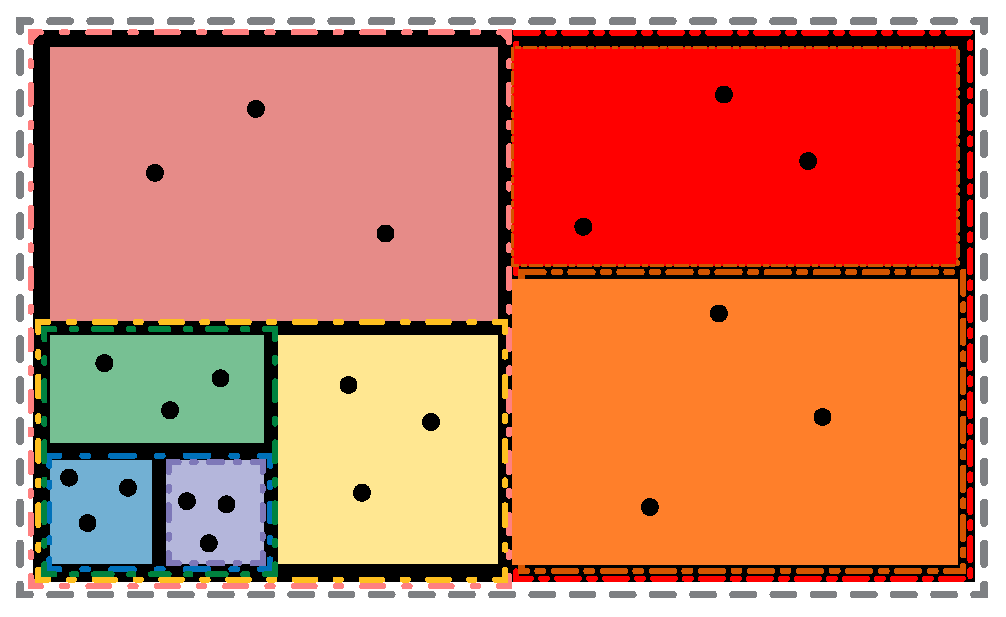
\includegraphics[width=\textwidth]{graphics/tree.eps}
                %\caption{A representation of the algorithm in real space, with the tree overlaid.}
                \label{fig:volumetree}
        \end{subfigure}
        ~ 
        \begin{subfigure}[b]{0.45\textwidth}
                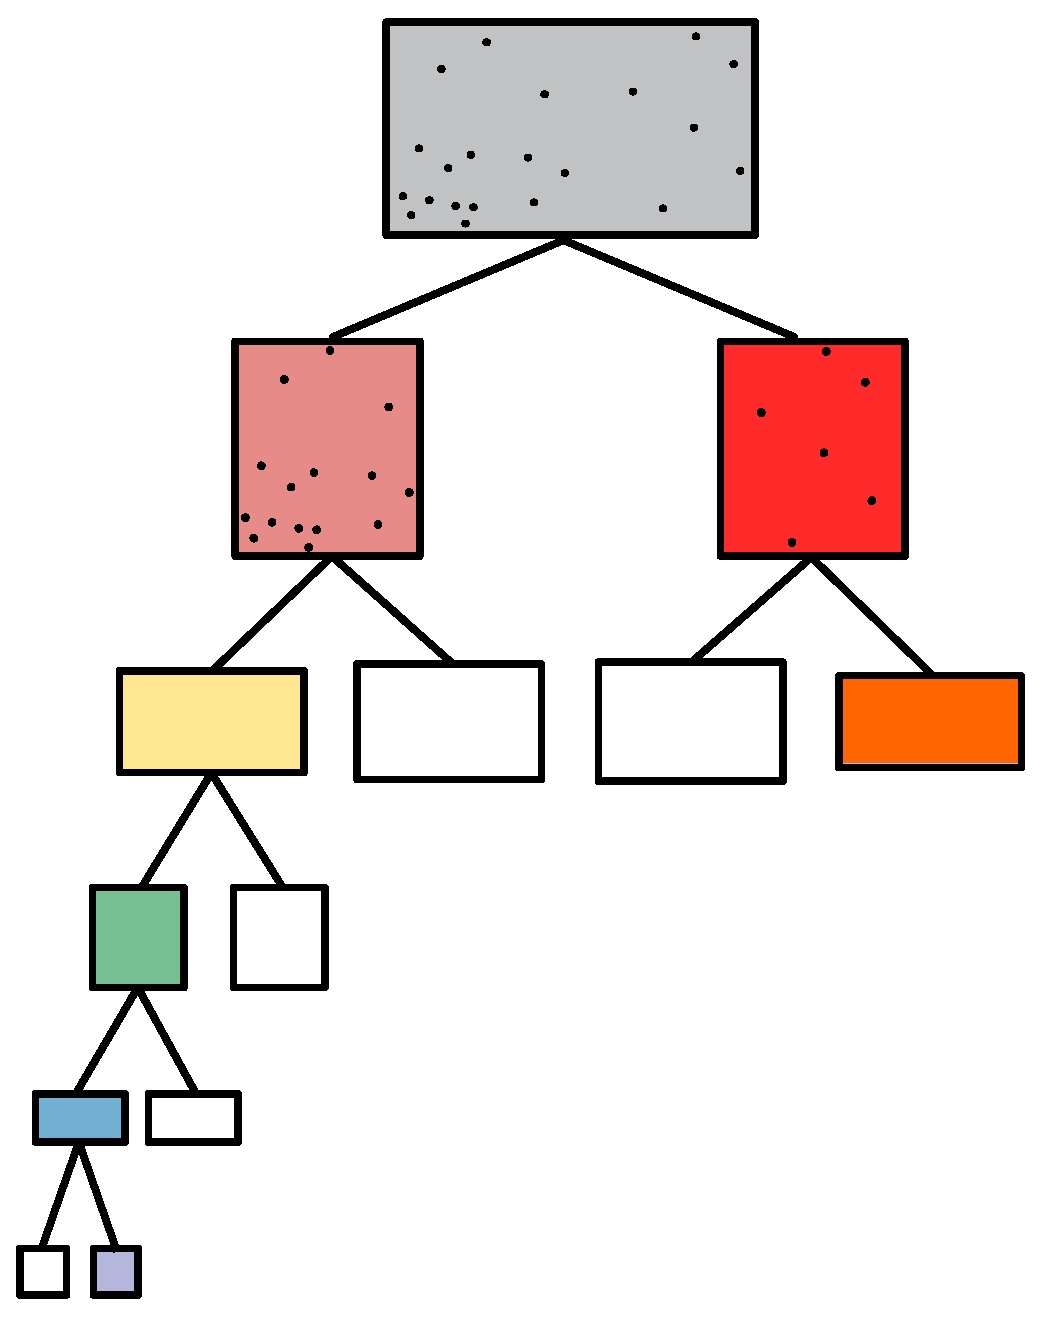
\includegraphics[width=\textwidth]{graphics/tree_memory.eps}
                %\caption{The colors correspond to the volumes on the left.}
                \label{fig:memorytree}
        \end{subfigure}
        \caption[Example of trees]{This is an example of a binary tree. The volume is represented by a tree node, and each volume is then split into two subvolumes, which are represented by two ``child'' nodes of the original node. This splitting can continue indefinitely on either side, making the tree an effective way at splitting volumes.}
        \label{fig:trees}
\end{figure}

Note that average properties of interest for radiation are total luminosity, center of luminosity, average density, average opacity, and the variance in opacity. The reasons for these properties will be discussed in section \ref{sec:absorption}.


%\section{Building a Radiation Tree}
%\label{sec:buildingtree}

%\begin{itemize}
%\item While the algorithm we present is general enough to work with any volume-filling tree, the following sections will introduce the algorithm as we have developed it. \textsc{Gasoline} uses a k-d tree for its gravity solver, and as such, our version of the algorithm uses this tree type in order to make use of existing tools in the code base.
%\item The recursive pseudocode for the tree-build is presented below (note - change to nice pseudocode format):
%	\begin{enumerate}
%	\item if number of data elements greater than n$_{\mbox{leaf}}$, partition data
%	\item recursively call build tree on each partition of the data set
%	\item else, if number of data elements less than n$_{\mbox{leaf}}$, calculate basic cell properties
%	\item After if statement, calculate accumulated cell properties (higher moments, etc)
%	\end{enumerate}
%\item In our case, the partition data step involves finding the longest axis of the data contained on the current node and dividing particles to the upper and lower halves of the midway point of that axis.
%\item Each volume and its corresponding list of particles is then passed recursively to the tree build function again. This terminates when build tree receives a list of particles that is sufficiently short (less than a user set parameter, n$_{\mbox{leaf}}$). At this point, basic cell properties such as center of luminosity and total luminosity are calculated.
%\item Once the leaf nodes have been calculated, more complicated average properties, such as higher moments, can be calculated by looping through all particles in the node. This applies to both leaf and interior nodes.
%\item The initial partition function does not require that the data be fully sorted, only that it be divided to either side of an intermediate value. This is an order n operation.
%\item The tree will be roughly of depth $\log(N)$, meaning that the partition will need to be performed $\log{N}$ times. Therefore, the tree build should scale as roughly $N\log{N}$.
%\item For radiation, average cell properties that are used are average density, average opacity, standard deviation of opacity, total luminosity, and center of luminosity.
%\item Note that we have calculated center of luminosity without taking into account absorption within the cell.
%\end{itemize}

\section{Exchanging Radiation}
\label{sec:exchangerad}

Once the tree has been built, calculating the radiation (gravity) at any particular point can be accomplished by traversing the tree structure, a process called a ``tree walk.'' First, a ``post-order'' tree walk is performed in which the children of a node are always checked before its sibling. The walk continues until it arrives at a leaf node, at which point the radiation (gravity) arriving at that leaf is calculated. This leaf node will be called the receiving leaf.

A second tree walk occurs during the radiation (gravity) calculation. We must check what cells are acceptable to interact with based on a particular criteria. Gravity calculations use what is called an opening angle criteria. The idea is that for any cell, if the cell takes up a sufficiently small solid angle on the sky, then the entire contents of the cell can be approximated as a single object located at the center of mass of the cell. In order to determine this, the simplest criteria to check is whether

\begin{equation}
\label{eq:openingangle}
\frac{b_{\mbox{max}}}{r} < \theta_{\mbox{crit}},
\end{equation}

where $\theta_{\mbox{crit}}$ is a user set parameter, $b_{\mbox{max}}$ is the largest extent of the cell, and r is the radius from the receiving cell to the cell in question. If a cell does not satisfy this criteria, it must then examine each child of the cell. If it does satisfy the criteria, then it can interact with that cell and move on to checking the next one. If a cell fails this criteria, but is a leaf node and cannot go down any further, then all particles within the lead node are interacted with individually. Note that in practice, it is more efficient to rewrite equation \ref{eq:openingangle} in terms of radius,

\begin{equation}
\label{eq:openingradius}
r_{\mbox{crit}} = \frac{b_{\mbox{max}}}{\theta_{\mbox{crit}}}.
\end{equation}

This process is illustrated graphically in figure \ref{fig:openinganglecriteria}. In this figure, Cell A is the receiving cell, and cells B, C, and D are cells to interact with. In this case, cell B fails the criteria, but cannot be opened any further and so the particles inside of B are interacted with individually. Cell C fails the criteria as well, but since it is not a leaf, each of its children are checked. Cell D passes the criteria, so the interaction is done with the center of luminosity of the cell. The interaction is depicted in figure \ref{fig:radexchange}.

\begin{figure}
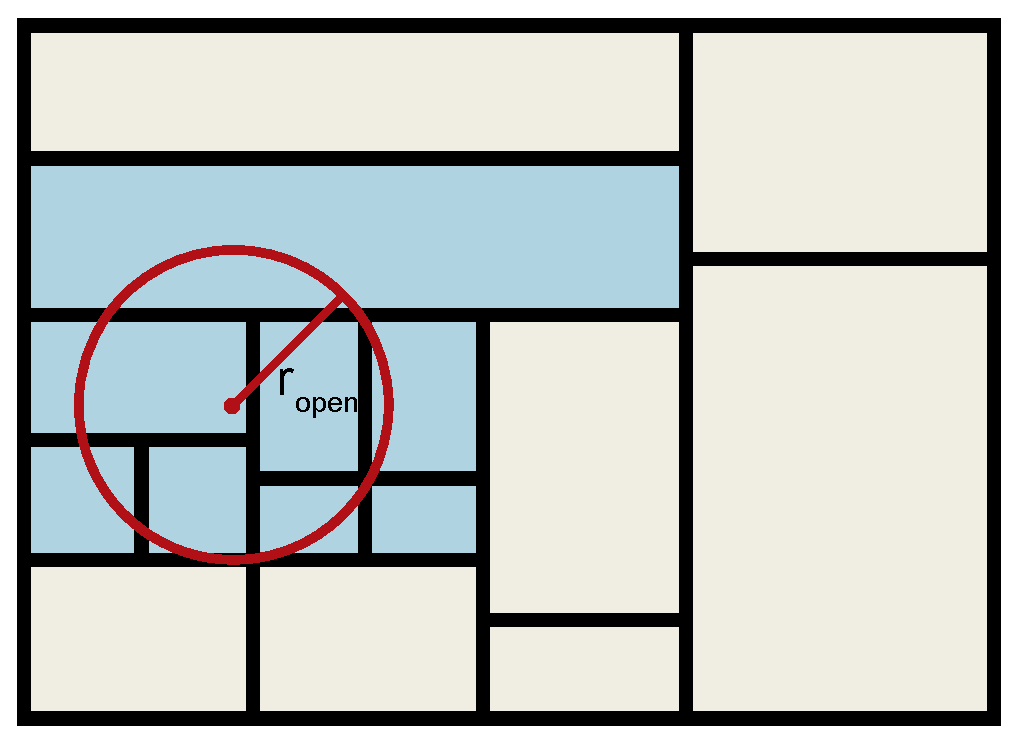
\includegraphics[width=\textwidth]{graphics/opening_angles.eps}
\caption[The opening angle criteria.]{Cell A in this image is the receiving cell, while cells B, C, and D are cells that A will receive flux from. Cell B is close enough so that it should be opened, but is a leaf and so it requires a direct $n^2$ summation. Cell C is close enough and is not a leaf, so it will have its two children checked for the same criteria (the left child will be too close, the right child will be acceptable to interact with). Cell D is not a leaf, but is sufficiently far away that leaf A can interact with the full cell.}
\label{fig:openinganglecriteria}
\end{figure}

\begin{figure}
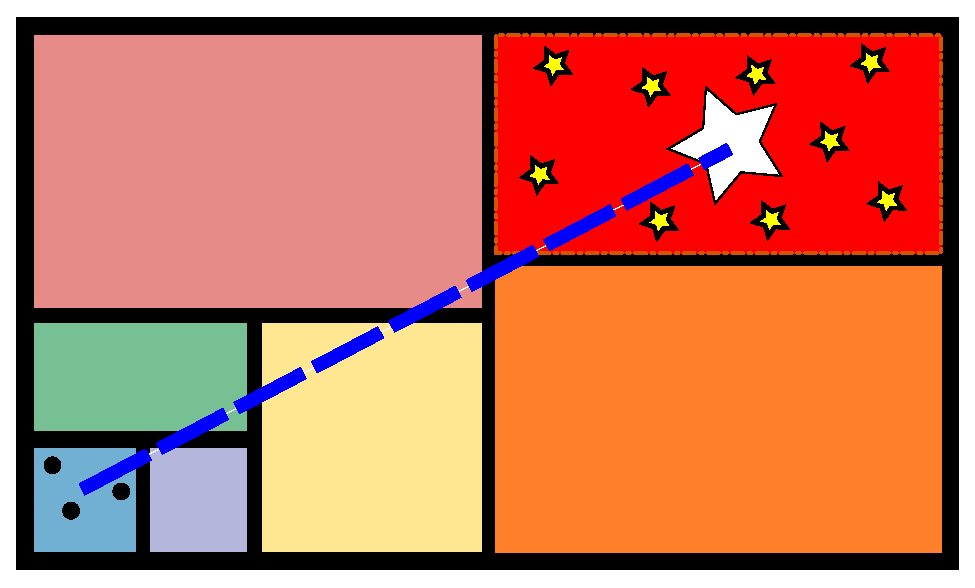
\includegraphics[width=\textwidth]{graphics/flux.eps}
\caption[The exchange of radiation.]{In this image, cell A is receiving radiation from cell B. Cell B is sufficiently far away that we can find the center of luminosities of all the sources inside of it, and calculate flux based on that single value rather than summing each one individually.}
\label{fig:radexchange}
\end{figure}

Once radiation has been calculated for the receiving leaf, we move on to the next leaf, which is accomplished by moving to the sibling if the current leaf is the left child of the parent node, or to the sibling of the parent node if we are the right child. An example radiation exchange is shown in figure \ref{fig:radexchange}.

The above algorithm will run in $N\log{N}$ time, as with gravity. However, unlike gravity, not all objects emit radiation. Thus, technically the more specific scaling is $N_{\mbox{sink}}\log{N_{\mbox{source}}}$. The slow growth rate of computation time with the number of sources makes the algorithm a very strong candidate for cosmological applications in which there are often similar numbers of star particles to gas particles. As was mentioned in chapter \ref{chap:radtransfer}, some codes have already made use of this basic idea \citep{gnedinAbel01,hopkins, kannanEt14}.

%\begin{enumerate}
%	\item Given a cell (starting with the root cell), check if the distance, r, from the current leaf to the cell is shorter than the opening radius (given by equation \ref{eq:openingradius}).
%	\item If r is shorter than the opening radius, the cell must be ``opened,'' meaning that we return to step 1, but now passing in each child node to check.
%	\item If r is longer than the opening radius, the cell is acceptable to interact with. The radiation may be calculated to the bucket using equation \ref{eq:bucketflux}. See figure \ref{fig:openinganglecriteria}.
%	\item In the case that the distance to the cell is smaller than the opening radius, and the node has no children (e.g. for leaves of the tree that are very spatially close to the receiving leaf), the interaction should not be approximated, and the direct n$^2$ summation over all particles in each leaf is performed.
%	\item Once radiation has been calculated from the current cell, the tree-walk is allowed to skip all children of the current cell and move on to its sibling or parent's sibling (parent's sibling in the case that we are the right-hand child of the parent node). 
%\end{enumerate}


%\begin{equation}
%\label{eq:bucketflux}
%F_{\mbox{bucket}} = \frac{L_{\mbox{tot}}}{4\pi r^2}e^{-\tau}
%\end{equation}

\section{Absorption}
\label{sec:absorption}

The algorithm presented in sections \ref{sec:buildingtree} and \ref{sec:exchangerad} assumes that no change to the radiation happens in between the sending and receiving cells. In gravity, this is acceptable because forces are not ``absorbed'' in any way. However, radiation tends to be absorbed and scattered by intervening material and thus the intensity of the radiation at a point is not only due to the sending source, but to all material in between the source and the sink. As was mentioned in the introduction of this chapter, we choose to omit scattering and focus only on absorption. The goal, then, is to find the optical depth between two interacting cells without adding significant computational cost. In order to accomplish this, we have developed the algorithm to make use of the tree during the optical depth calculation as well.

The crucial point to the algorithm lies in the fact that for any two interacting cells, there exists a common parent node above them. Thus, all intervening space between the cells must lie within the subtree in which the common parent is the root [should add figure to show this]. If we traverse up the depth of the tree (hereafter referred to as a tree climb) from each interacting node to the common parent node, we will have performed roughly $\log(N)$ extra operations per interaction on average. If we do no other work than this, then our scaling for radiative transfer changes to $N_{\mbox{sink}}\log{N_{\mbox{source}}}\log{N}$. While the extra factor of $\log{N}$ is certainly worth noting, it does not tend to increase scaling by a significant amount. Our goal then becomes to perform $\mathcal{(1)}$ amount of work during this additional tree climb.

As was mentioned in section \ref{sec:treestruct}, the tree records average properties as it is built, including average opacity and density. Referring to the definition of optical depth (equation \ref{eq:opticaldepth}), we see that we can get an estimate of the optical depth through a cell by using the average opacity, the average density, and finding the segment of the ray inside the cell,

\begin{equation}
\label{eq:averageopticaldepth}
\tau_i = \bar{\rho}\bar{\kappa}ds,
\end{equation}

where $\tau_i$ is the optical depth in cell i, $\bar{\rho}$ is the average density in the cell, $\bar{\kappa}$ is the average opacity, and $ds$ is the length of the ray segment contained in the cell.

At each higher cell during the tree climb, we obtain a larger representative volume from that cell. The new volume contains the previous volume as well as a new contribution from the previous cell's sibling. This sibling's volume may or may not lie on the vector connecting the two interacting cells. This can be determined by calculating the distance to the edge of the current volume along the vector from the centers of the original interacting cells, an operation that takes $\mathcal{(1)}$ time.

At each new parent cell, if the calculated line segment is longer than the accumulated distance so far, than the difference is the amount of the ray contained in the sibling cell. By recording this new line segment, the average density of the cell, and the average opacity of the cell, we have everything needed to calculate the optical depth of the line segment. By summing the optical depth of each line segment, we will have obtained the full optical depth between the interacting cells in order $log{N}$ time, giving a full scaling of $\mathcal{O}(N_{sink}\log(N_{source})\log(N))$. The algorithm is depicted graphically in figure \ref{fig:absorption}.

%\begin{figure}
%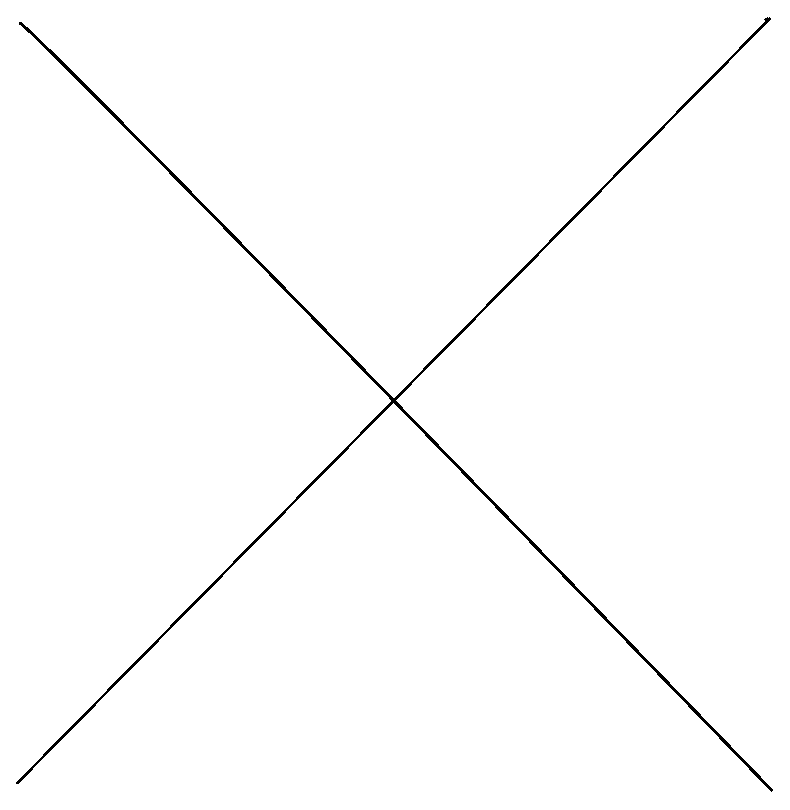
\includegraphics[width=\textwidth]{graphics/placeholder.eps}
%\caption{}
%\label{fig:absorption}
%\end{figure}

\begin{figure}
        \centering
        \begin{subfigure}[b]{0.45\textwidth}
                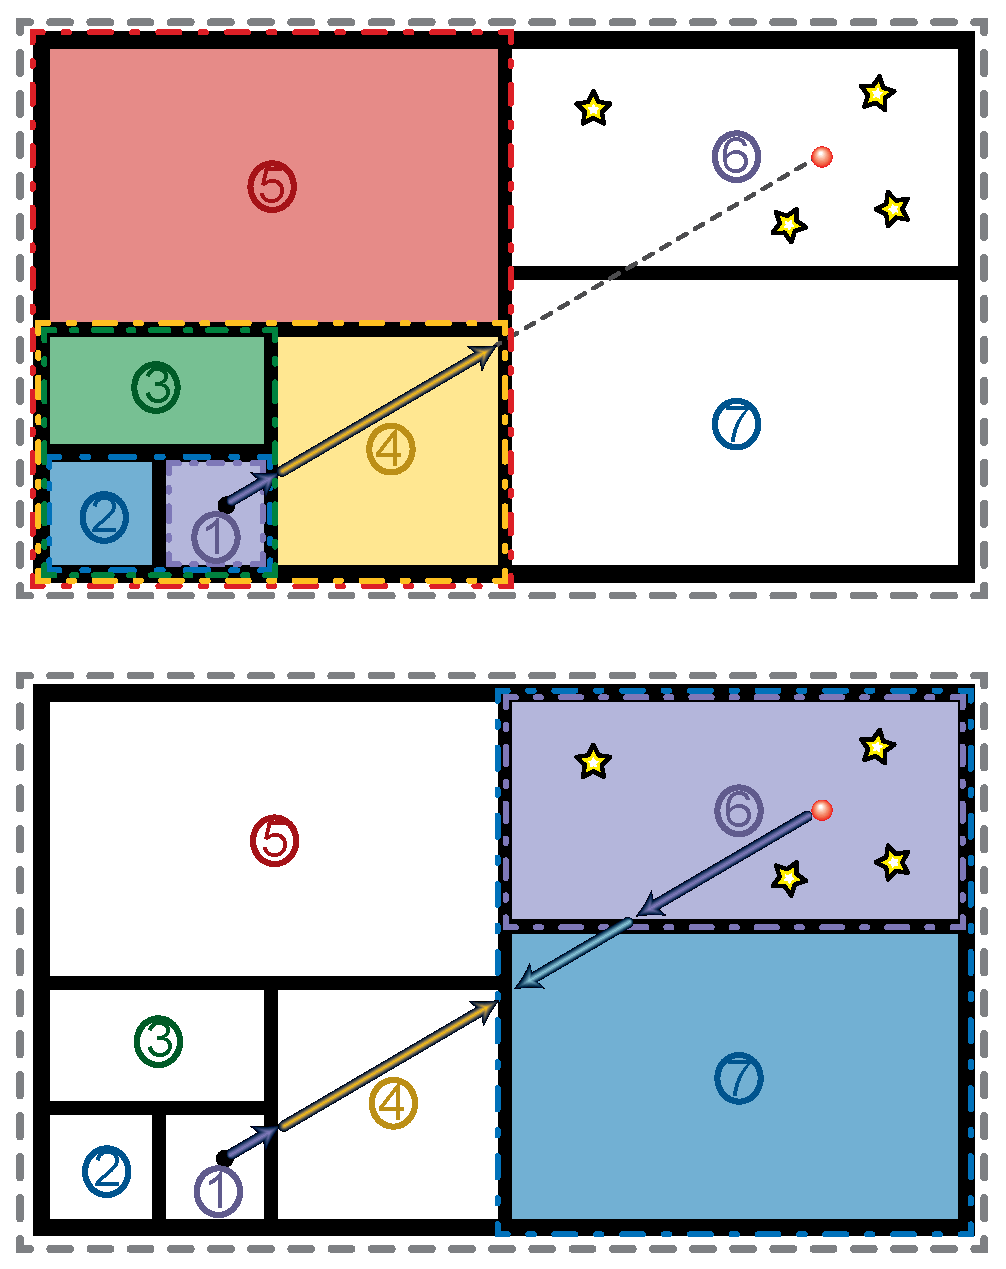
\includegraphics[width=\textwidth]{graphics/RT_algorithm.eps}
                \caption{A representation of the algorithm in real space, with the tree overlaid.}
                \label{fig:treeclimb}
        \end{subfigure}
        ~ 
        \begin{subfigure}[b]{0.45\textwidth}
                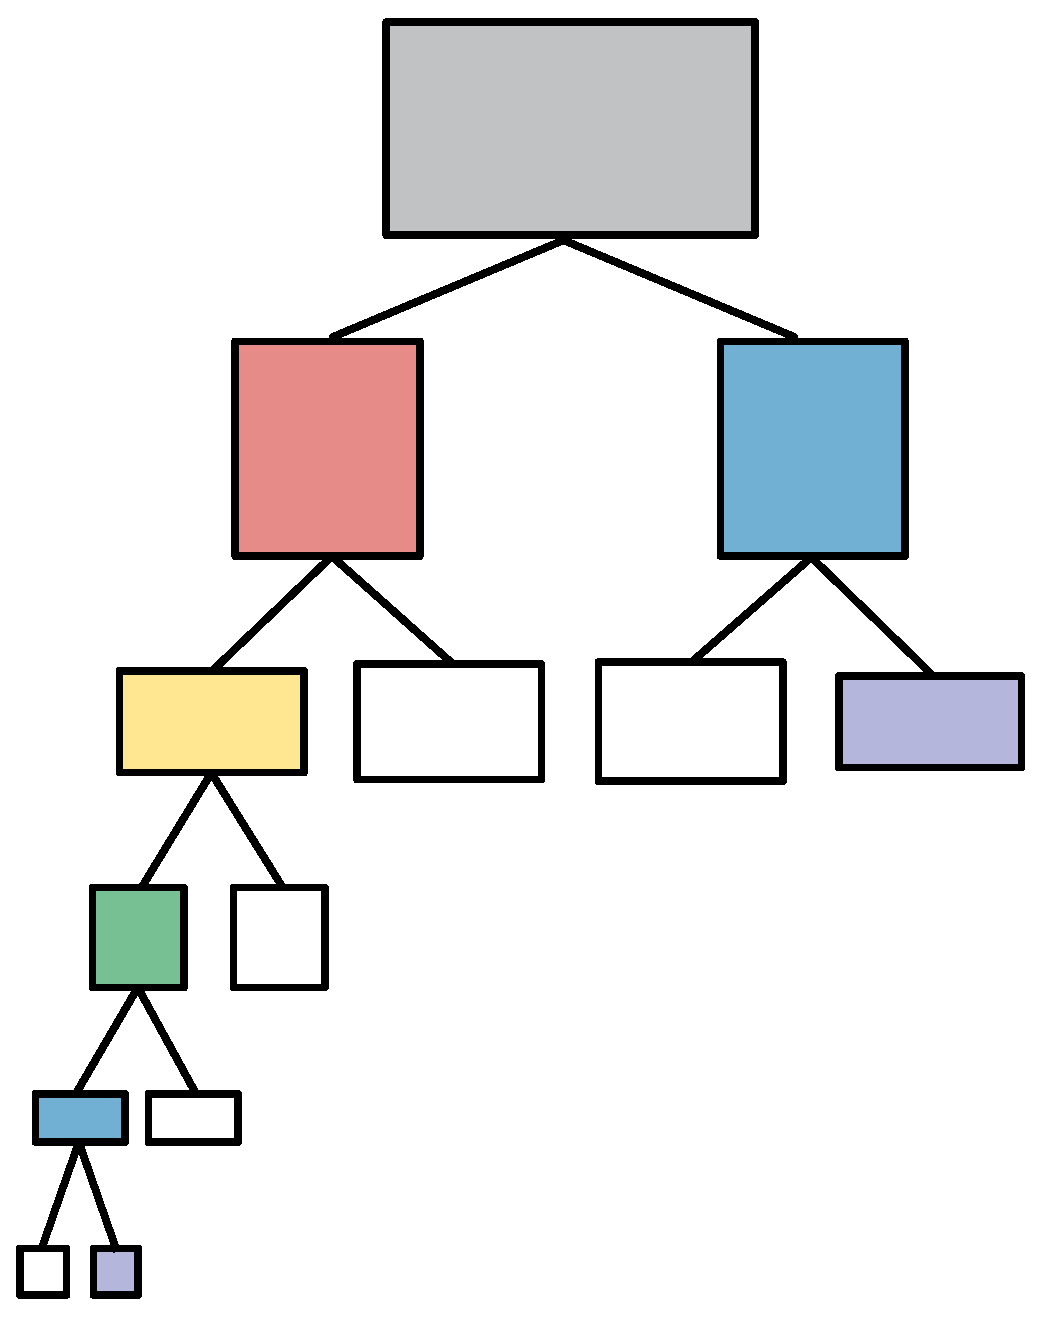
\includegraphics[width=\textwidth]{graphics/RT_tree.eps}
                \caption{The colors correspond to the volumes on the left.}
                \label{fig:absorptiontree}
        \end{subfigure}
        \caption[The absorption algorithm.]{The absorption algorithm.}
        \label{fig:absorption}
\end{figure}



\section{Refinement}
\label{sec:refinement}

While section \ref{sec:absorption} introduces a very fast algorithm for calculating a radiation field, it relies heavily on the geometry of the underlying tree. In volumes with very smooth density and opacity, the above algorithm performs very well. However, in cases with sharp density or opacity gradients, the gradient is discretized into widths of order the cell size at the current tree depth. This can become problematic, causing the tree structure to be imposed into the calculated radiation field. In order to solve this, we introduce a refinement process to the algorithm that allows a descent back down the tree during the tree climb in order to obtain a more detailed description of the medium.

Refinement is a fairly straightforward addition to the algorithm. At the point where the average properties of the cell would normally be considered, we simply check if the current cell passes a refinement criteria. If the cell passes the criteria to refine, rather than recording the average properties, we recursively check the children of the section of the tree we did \emph{not} ascend from. Once we arrive at a cell that fails the criteria to refine (or at a leaf and can no longer refine), we record the line segment within the cell and the average properties as normal, and return up the recursive call. See figure \ref{fig:refining} for a visual representation.

\begin{figure}
        \centering
        \begin{subfigure}[b]{0.45\textwidth}
                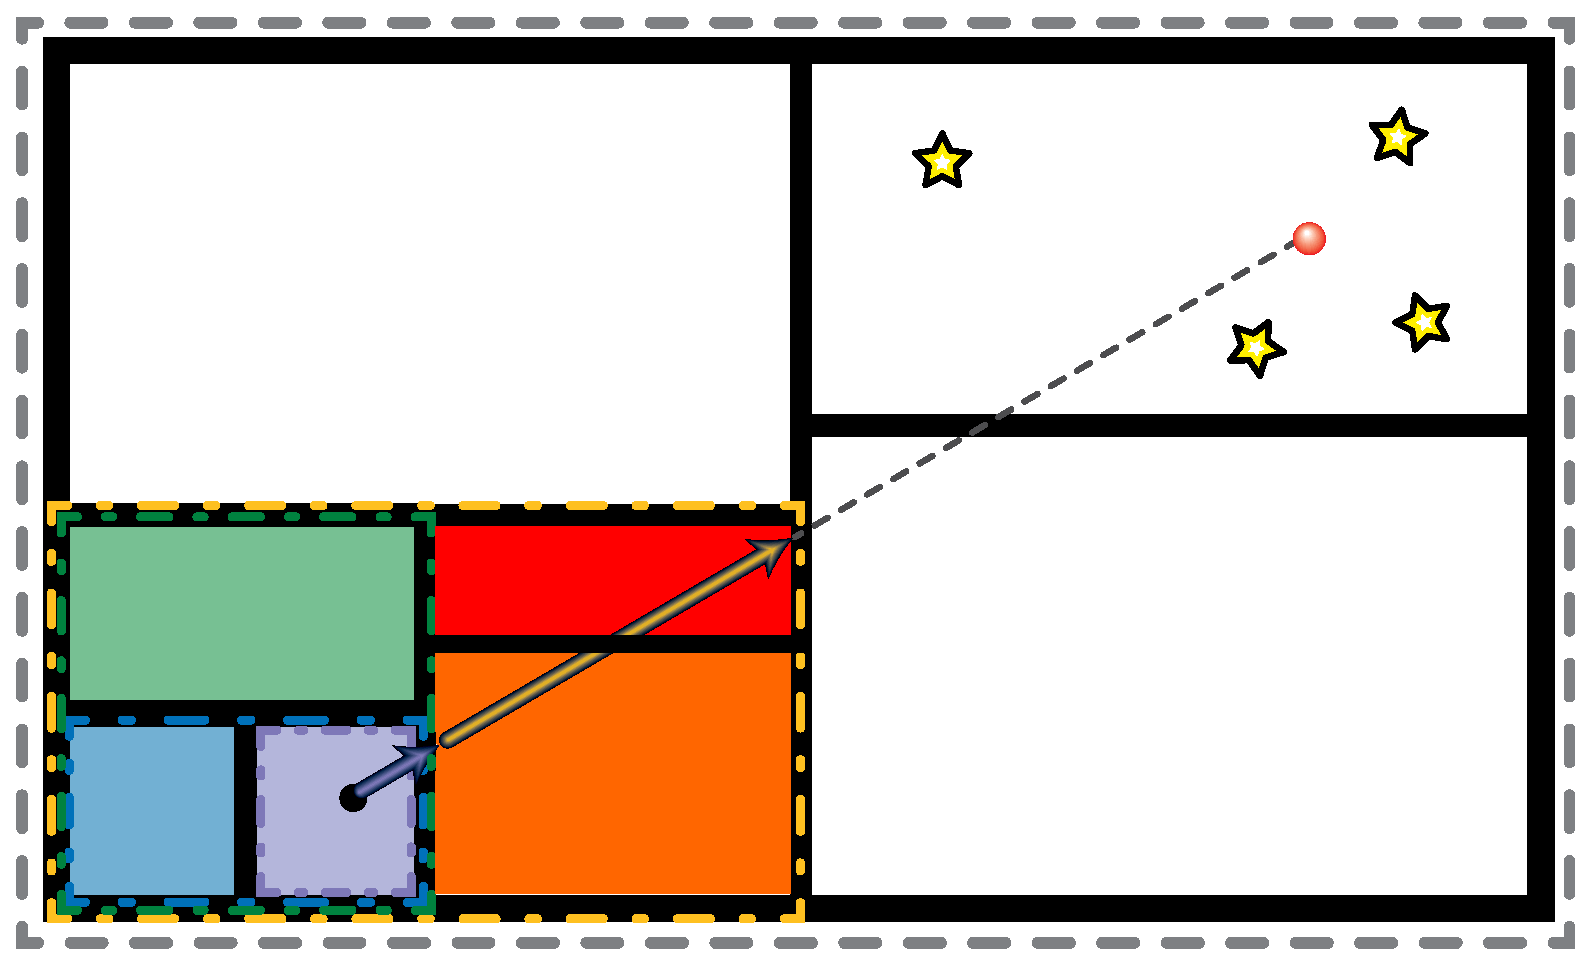
\includegraphics[width=\textwidth]{graphics/refinement.eps}
                \caption{The tree splits the line segment into the red and orange sections.}
                \label{fig:refinetree}
        \end{subfigure}
        ~ 
        \begin{subfigure}[b]{0.45\textwidth}
                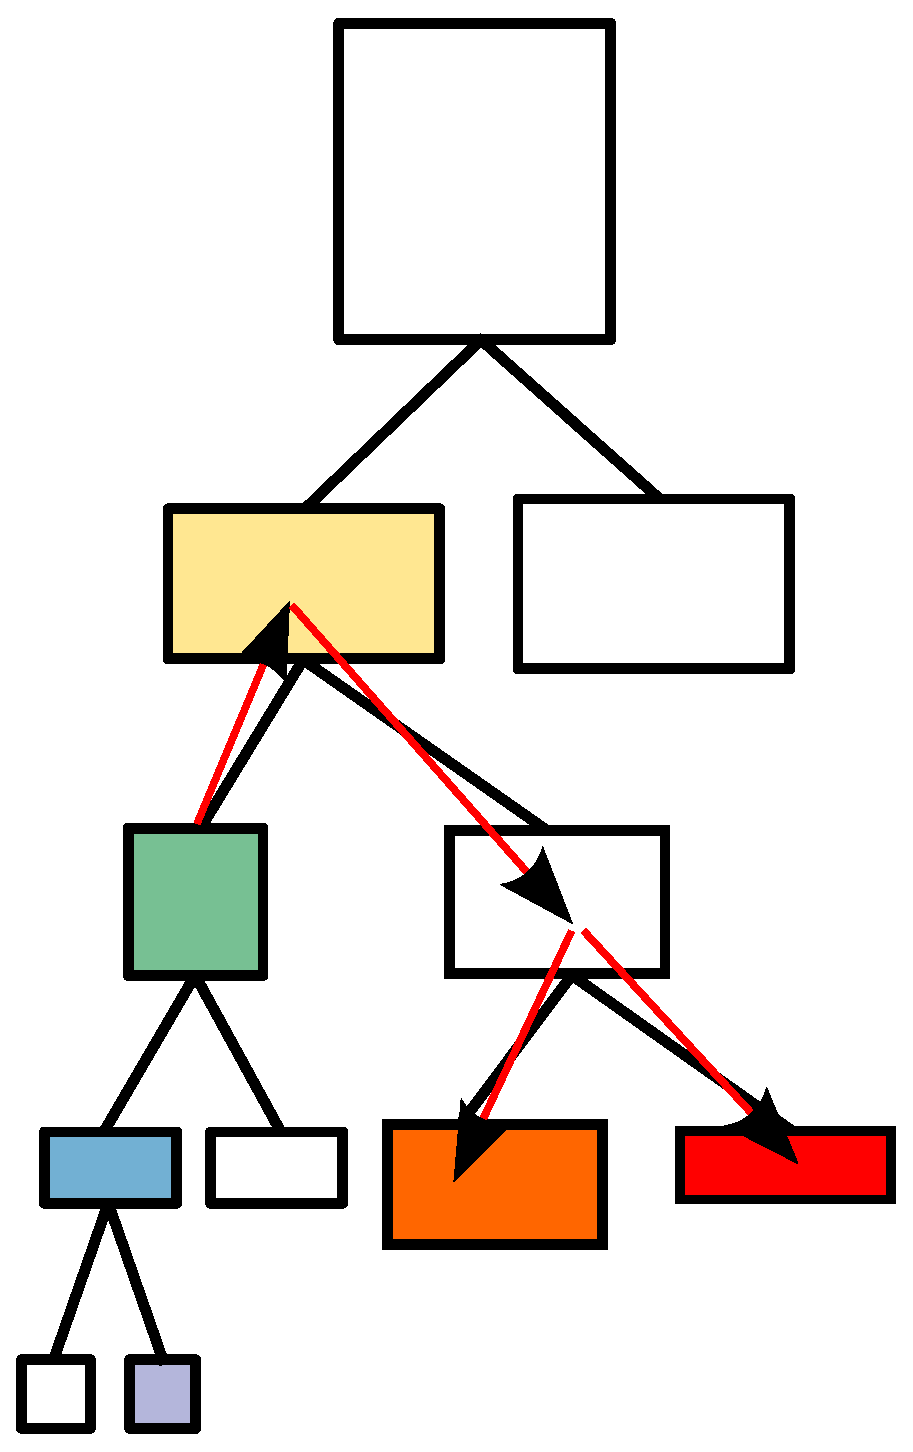
\includegraphics[width=\textwidth]{graphics/refine_memory.eps}
                \caption{The colors correspond to the volumes on the left.}
                \label{fig:refinememory}
        \end{subfigure}
        \caption[Refinement during the absorption algorithm.]{When the line segment is too rough in some physical sense, refinement can be triggered. Visually, the algorithm descends back down the tree the opposite direction it came from until the criteria to refine is no longer satisfied or until a leaf is reached.}\label{fig:refining}
\end{figure}

The specific refinement criteria has deliberately been left vague until this point. In principle, one can refine on any cell property desired. Ideally, the criteria should be true when an average opacity in a region may not be accurate to the true distribution, such as a clumpy medium. In our testing, we have decided to use an opacity refinement criteria. Within any cell, if a constant times the standard deviation of the average opacity is larger than the average opacity, the cell is refined. We find this produces a reasonable amount of refinement in code tests [Need to update this]. Note that this is not necessarily the most computationally ideal criteria for physical simulations. It would be wise not only to look at the variation in opacity, but also the absolute value. In cases where the optical depth is very high, most of the radiation will be absorbed anyway, and the algorithm can be terminated since this particular ray yields a negligible flux of photons to the receiving cell.

If very high accuracy is required, the refinement routine is flexible enough that sub-leaf refinement is possible. If a leaf was reached during refinement and still passed the criteria to be refined on, the individual particles inside the cell could be considered. A ray tracing scheme through the cell similar to SPHRay \citep{altayEt08} could be performed. The machinery to do this ray trace is already established for use within the receiving and sending cells (see section \ref{sec:resolvingleaves} and figure \ref{fig:particletracing}). However, this has not currently been tested since it leaves the regime of low computational expense.

\section{Resolving the Receiving Cells}
\label{sec:resolvingleaves}

During testing, we ran into issues with ionization fronts ``stalling'' in certain cells. If a sharp ionization front is passing through a receiving leaf node, then the effects of averaging can cause issues if the optical depth of the bucket is of order unity or higher. To understand why, consider the following scenario.

Consider an ionization front that has passed halfway through a leaf node (half of the particles are ionizaed, half are not). The average opacity will be $\kappa/2$, where $\kappa$ is the opacity of the unionized particles. The ionized particles will use an opacity that is much too large, therefore reducing the flux that particles at the ``rear'' (further from the direction of radiation) of the leaf see. This means that particles at the rear of the leaf are harder to ionize than at the front, and the propagation speed of the front is drastically reduced.

In order to combat this, more detailed tracing is required \emph{only in the receiving leaf}. This is easily accomplished by implementing a scheme similar to SPHRay \citep{altayEt08}. In this method, all particles in a cell are projected down to the ray, and an impact parameter, b, is calculated. See figure \ref{fig:particletracing}.

\begin{figure}
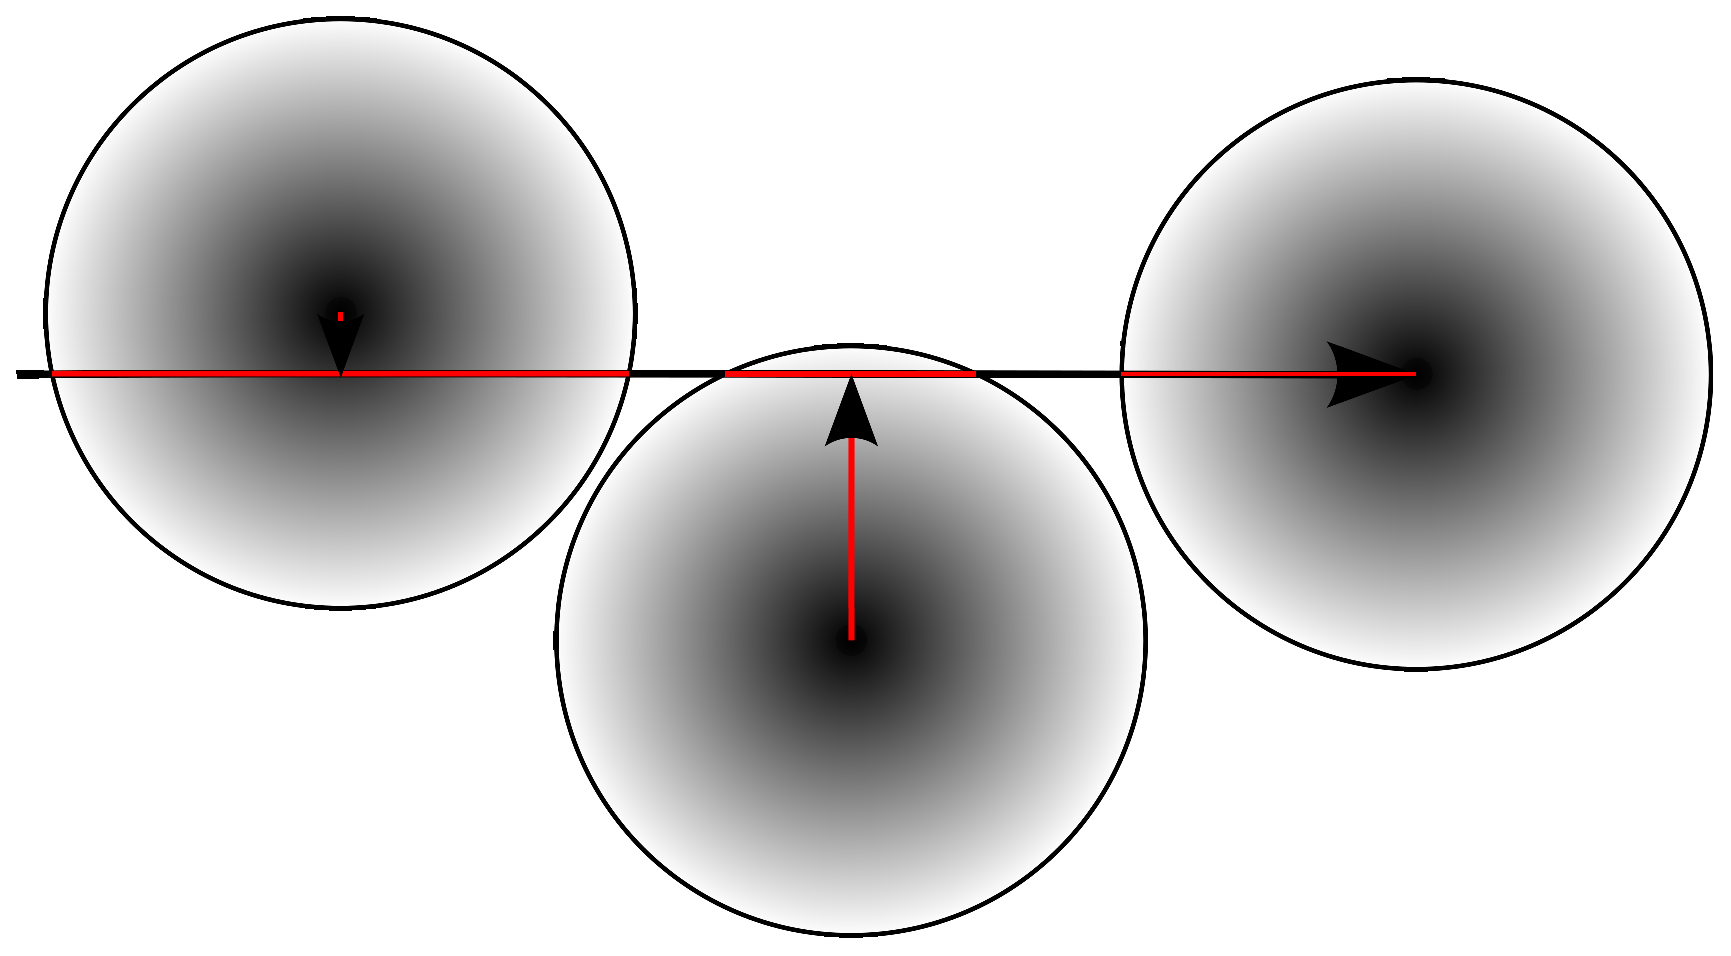
\includegraphics[width=\textwidth]{graphics/raytrace.eps}
\caption[Ray tracing schemes for receiving cells.]{The ray tracing scheme, similar to \citet{altayEt08}. In this scheme, the photons are diminished by the optical depth along each particle's density field.}
\label{fig:particletracing}
\end{figure}

Since the density field of a particle varies with radius from the particle due to the smoothed nature of SPH, an integral over the kernel must be performed. Thus, equation \ref{eq:opticaldepth} changes to

\begin{equation}
\label{eq:kernelintegral}
\tau_{\nu} = (m_i\int W)\kappa ds,
\end{equation}

where $(m_i\int W)$ represents the effective density along the particular ray, and $ds$ is the section of the ray intersected by the particle's smoothing length.

Introducing the ray tracing machinery for the above purpose also creates the ability to ray trace within leaves during the refine mentioned in section \ref{sec:refinement}. In principle, this means the code can easily be forced into a full ray trace if this behavior is desired.

%\subsection{High Optical Depth Particles}
%\label{sec:hightau}
%
%High tau particles are problematic. This is how we deal with them...

%\section{Periodicity}
%\label{sec:periodicity}
%
%Move to future work?

\section{Cosmological Background Radiation}
\label{sec:cosmobackground}

In order to do cosmological simulations properly, we must account for the radiation coming from the rest of the universe outside of the simulation volume. Most current codes apply a constant UV field to the entire box, essentially the lowest order approximation possible. Some specialized codes (e.g. URCHIN \citet{altayTheuns13}) do inverse ray tracing from sinks to the edge of a box, where a background flux is assumed to be coming from. Other, such as TRAPHIC \citep{pawlikSchaye08} or OTVET \citep{petkovaSpringel09}, allow their ray trace to be periodic, so that photons leaving the box represent photons coming in from the other side.

While our scheme is perfectly capable of doing a periodic treatment, we have opted to set up a number of ``background sources.'' ``Background'' particles are distributed on the surface of a sphere at the very edge of the simulation (or larger if required) and the number of sources can be varied to match the required angular resolution of the background. Finding the flux at the center of a sphere of sources is a problem akin to Newton's Shell Theorem. However, because the flux doesn't cancel like force, the solution does not work out the same. Instead, the solution is

\begin{equation}
\label{eq:shellflux}
F = K\left[ \log{R+r} - ln(R-r) \right],
\end{equation}

where $K$ is a constant, $R$ is the radius of the sphere, and $r$ is the radius the flux is being measured at. The shape of this function can be seen in figure \ref{fig:backgroundflux}, where we have plotted flux vs radius for a cube of particles.

\begin{figure}
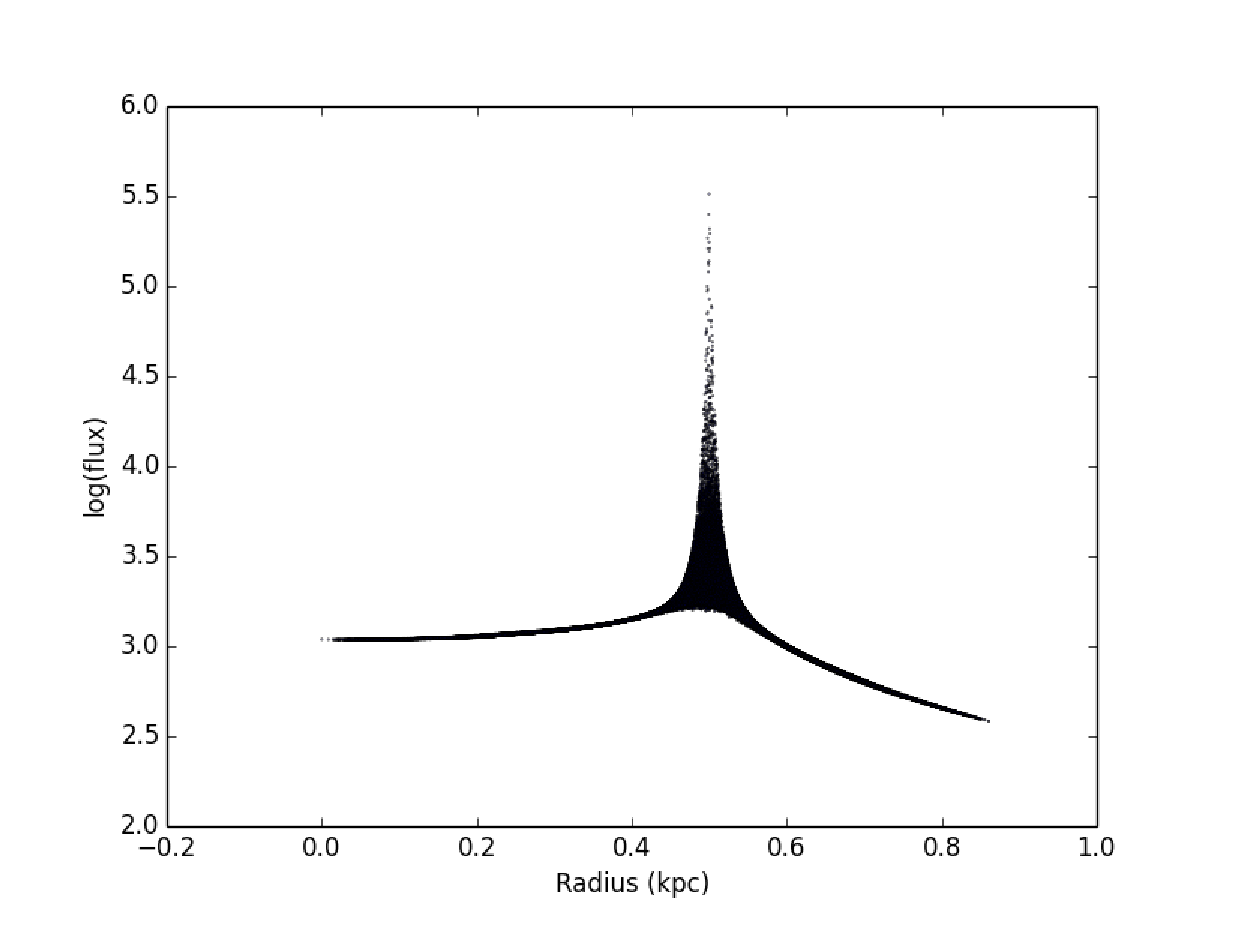
\includegraphics[width=\textwidth]{graphics/backgroundflux.eps}
\caption[Flux due to the cosmological background.]{The distribution of flux particles receive due to cosmological background particles when distributed in a sphere at the edge of the box. Note that value of the flux at the center can be easily scaled by simply scaling the luminosity of all sources on the sphere.}
\label{fig:backgroundflux}
\end{figure}

We note that due to the logarithms, the flux is nearly constant at small radii. Since most cosmological zoom simulations only consider gas at a fairly small radius, this setup of background sources is an acceptable method to providing a cosmological background flux. We simply require that the sources be placed at a large enough radius to ensure all gas particles are at a radius much smaller than the radius of the sphere.

The benefit of this method is that we can use all of the existing RT machinery described in the previous sections. The background particles are treated as normal sources and the algorithm proceeds as normal. There is no need to create periodic copies of the simulation volume.

%\section{Cosmological Effects}
%\label{sec:cosmoeffects}
%Move this section to ``future plans'' section?
%
%\subsection{Cosmological Redshift of Radiation}
%\label{sec:redshiftingradiation}
%
%
%\subsection{Accounting for a Finite Speed of Light}
%\label{sec:finitespeedoflight}
%
%Move this section to ```future plans'' section?

\section{Summary of the Algorithm}
\label{sec:algorithmsummary}

We have presented a flexible and computationally inexpensive algorithm for calculating the radiation field within a simulation. It is flexible enough to allow a wide range of accuracy depending on the application. Scaling starts at  $N_{sink}\log{N_{source}}\log{N}$ and approaches that of ray tracing [check this...] when the algorithm is tuned to that level of refinement.

Because radiation is transferred instantaneously, the speed of light does not become a limiting factor to time steps. If ionization dynamics are important, then the propagation of the ionization front becomes the limiting time step. If only end behavior is required, then the there is very little the algorithm does to limit the time step.

The algorithm is independent of wavelength or even number of wavelengths. The algorithm need only perform the tree walk and tree climb a single time in order to obtain the line segments in each cell. Performing different wavebands simply equates to recording multiple average opacities. This enables multi-band radiative transfer at no additional cost.

However, it is important to keep in mind the limitations and assumptions of this algorithm.

Photons are not explicitly conserved. In order to save computational time, we can not keep track of the photons deposited in intervening material during an exchange. We obtain an optical depth and simply assume that the photons lost in the process have been deposited in the intervening material. When the intervening material is the receiving bucket at a later point in the algorithm, it should receive roughly the correct number of photons due to a similar initial segment.

Light is transferred instantaneously, meaning that photon fronts could travel faster than allowed, and that sinks could receive photons from a source too far away to have sent photons there yet.

[Add more here. Compare to codes from section 2.]